\documentclass[tikz,border=10pt]{standalone}
\usepackage{tikz}
\usetikzlibrary{arrows.meta}

\begin{document}

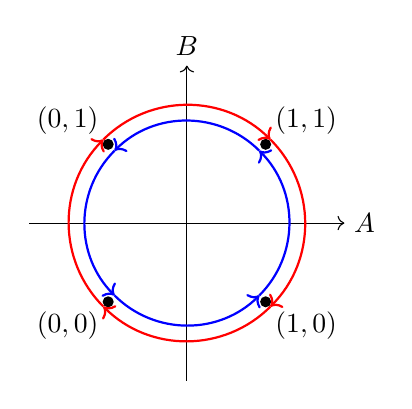
\begin{tikzpicture}[scale=2]

  % Axes through the center
  \draw[->] (-1,0) -- (1,0) node[right] {$A$};
  \draw[->] (0,-1) -- (0,1) node[above] {$B$};

  % Points (translated by (-0.5,-0.5))
  \fill (-0.5,-0.5) circle (1pt) node[below left] {$(0,0)$};
  \fill ( 0.5,-0.5) circle (1pt) node[below right] {$(1,0)$};
  \fill ( 0.5, 0.5) circle (1pt) node[above right] {$(1,1)$};
  \fill (-0.5, 0.5) circle (1pt) node[above left] {$(0,1)$};

  % Radius of arcs
  \def\rb{0.65}
  \def\rr{0.75}

  % Counter-clockwise arcs (blue)
  \draw[blue, thick, ->] (0,0) ++(-135:\rb) arc (-135:-45:\rb);
  \draw[blue, thick, ->] (0,0) ++(-45:\rb)  arc (-45:45:\rb);
  \draw[blue, thick, ->] (0,0) ++(45:\rb)   arc (45:135:\rb);
  \draw[blue, thick, ->] (0,0) ++(135:\rb)  arc (135:225:\rb);

    % Counter-clockwise arcs (blue)
  \draw[red, thick, <-] (0,0) ++(-135:\rr) arc (-135:-45:\rr);
  \draw[red, thick, <-] (0,0) ++(-45:\rr)  arc (-45:45:\rr);
  \draw[red, thick, <-] (0,0) ++(45:\rr)   arc (45:135:\rr);
  \draw[red, thick, <-] (0,0) ++(135:\rr)  arc (135:225:\rr);

\end{tikzpicture}

\end{document}
